\documentclass[a4paper]{article}

%\usepackage{fullpage}
\usepackage[14pt]{extsizes}			% размер шрифта
\usepackage{cmap}				% поиск в PDF
\usepackage[T2A]{fontenc}			% кодировка
\usepackage[utf8]{inputenc}			% кодировка исходного текста
\usepackage[english,russian]{babel}	% локализация и переносы
\usepackage{mathtools}			% математический пакет (включает ams)
\usepackage[thinc]{esdiff}			% производные
\usepackage{graphicx}				% изображения
\usepackage{listings}				% програмный код
\lstset{
	numbers=left               
}

\author{Бартая Нодари ФМ-101}
\title{ОТЧЁТ\\ Компьютерные технологии в\\ науке и образовании\\ Задание № 5}
\date{\today}

\begin{document}

\maketitle
\newpage
\section{Постановка задачи}

Требуется рассчитать траекторию движения электрона в скрещенных
постоянных магнитном и электрическом полях. 
С компонентами $\mathbf{E}=(E_x, 0, 0)$, $\mathbf{B}=(0, 0, B_z)$ и напряженностями 10 А/м и 10 В/м  соответственно. 
Начальная скорость электрона $\mathbf{v}_0$ направлена перпендикулярно вектору напряженности магнитного поля и составляет 10 см/с.
Геометрия задачи представлена на рисунке ниже.%\ref{problem} (стр. \pageref{problem}).

\begin{figure}[h]\label{problem}

	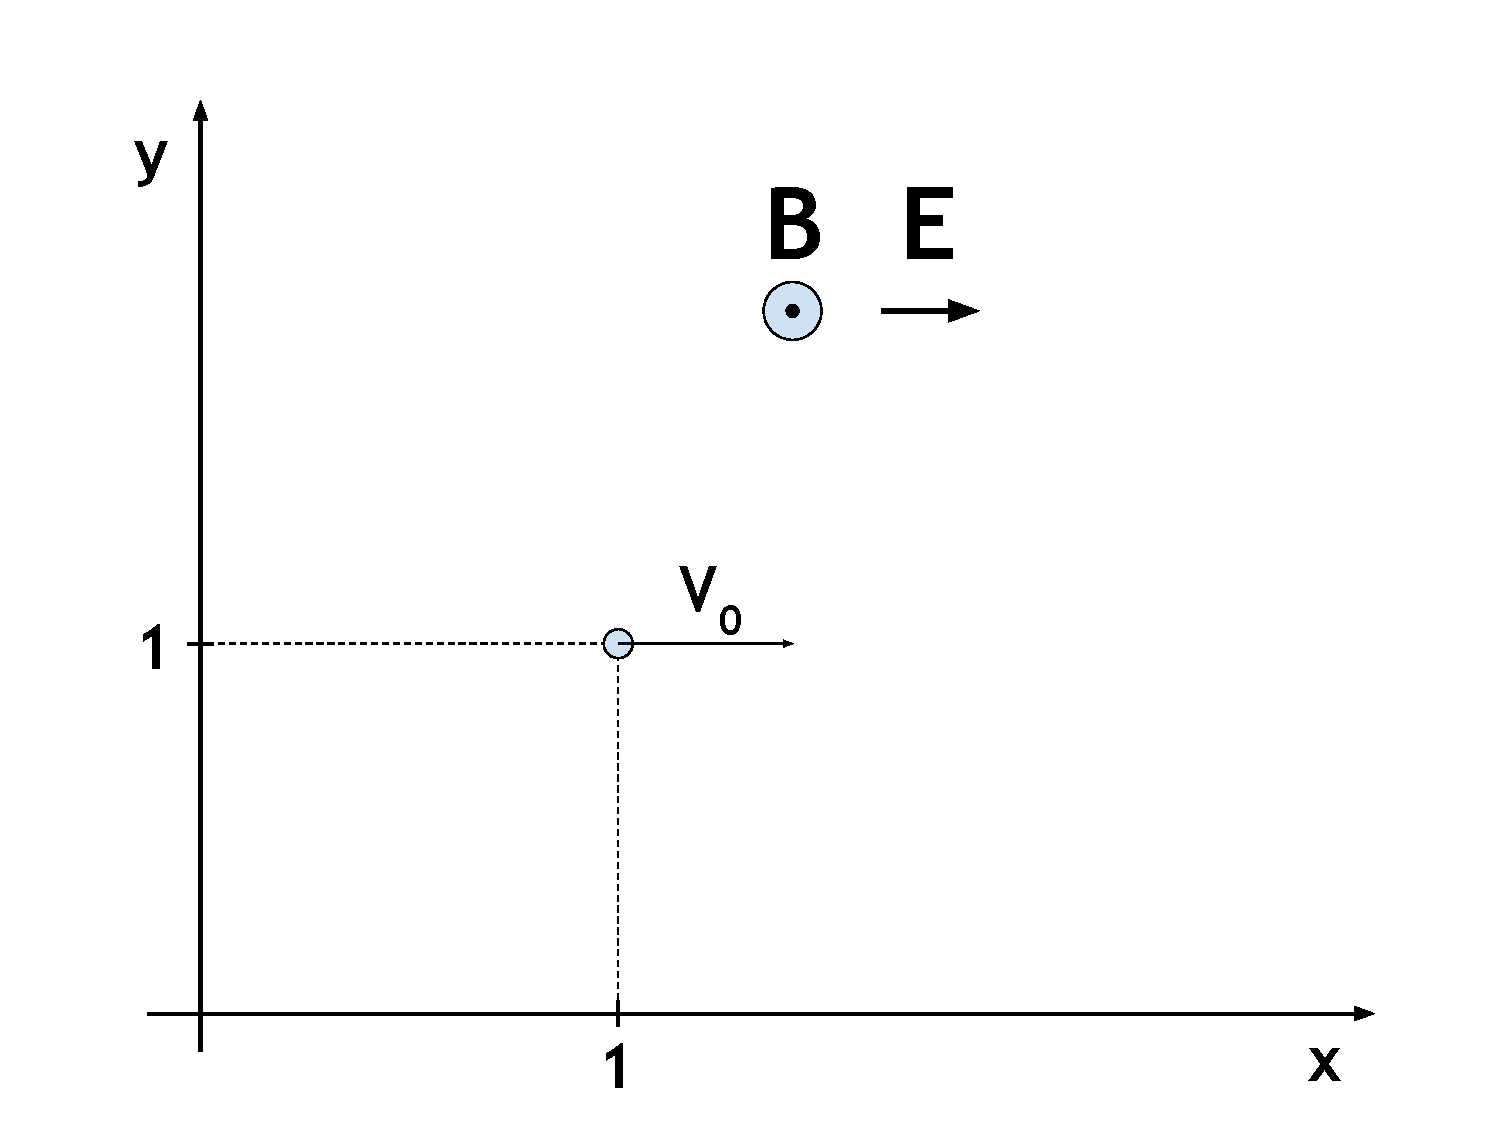
\includegraphics[width=\textwidth]{problem.pdf}
	\caption{Электрон в электромагнитном поле. Геометрия задачи, начальные условия.}
\end{figure}

\section{Аналитическое решение}
Решение будем искать в нерелятивистском приближении, то есть скорость движения электрона много меньше скорости света. Тогда, согласно второму закону Ньютона уравнение движения электрона имеет вид:
\begin{equation}\label{motion}
m\diff{\mathbf{v}}{t} = \mathbf{F},
\end{equation}
где $m$ - масса электрона, $\mathbf{v}$ - его скорость, $\mathbf{F}$ - действующая сила.

В элетромагнитном поле на заряженные частицы действует сила Лоренца:
\begin{equation}\label{lorenz}
\mathbf{F} = e \mathbf{E} + \frac{e}{c}\left[\mathbf{vB}\right],
\end{equation}
где $e$ - заряд частицы, $с$ - скорость света, $\mathbf{E}$ и $\mathbf{B}$ - напряженности электрического и магнитного поля, соответственно.

Уравнение движения \eqref{motion} относится ко классу дифференциальных уравнений с разделяющимися переменными. Таким образом, мы можем проинтегрировать уравнение движения и получить зависимость скорости от времени.

\begin{equation}\label{intmotion}
\int \mathrm{d}v =\int e \mathbf{E} + \frac{e}{c}\left[\mathbf{vB}\right] \, \mathrm{d}t
\end{equation}

Заряд частицы, скорость света и напряженности полей - постоянные величины. В этом случае, можно записать выражения для компонент скоростей в проекциях на оси координат:

\begin{equation}\label{velocity_components}
\begin{aligned}
v_x = v_{0x} + \left[ e E_x + \frac{e}{c} \left( v_y B_z - B_y V_z \right) \right] t \\
v_y = v_{0y} + \left[ e E_y + \frac{e}{c} \left( v_x B_z - B_x V_z \right) \right] t \\
v_z = v_{0z} + \left[ e E_z + \frac{e}{c} \left( v_x B_y - B_x V_y \right) \right] t
\end{aligned}
\end{equation}

Скорость, по определению, $\mathbf{v} = d\mathbf{r}/dt$, где $\mathbf{r}$ - радиус вектор положения частицы в пространстве. Подставив уже выведенные выражения для компонент скоростей и проинтегрировав аналогичным образом получим выражения для координат частицы:




\section{Численное решение}

Согласно уравнениям \eqref{motion}, \eqref{lorenz} численное решение для координаты частицы и скорости её движения в зависимости от времени будем искать для следующей системы дифференциальных уравнений первого порядка в соответсвии с геометрией задачи \ref{problem}.

\begin{equation}
	\begin{cases}
		\dot{v_x} \diffp{v_x}{t} = \left[eE_x + \dfrac{e}{c}\left(v_yB_z\right)\right]m^{-1}	
											& 	v_x(0) = 10 \\
		\dot{v_y} = \dfrac{e}{mc} v_x B_z	&	v_y(0) = 0 \\
		\dot{r_y} = v_y						&	r_x(0) = 1 \\
		\dot{r_y} = v_y						&	r_y(0) = 1 
	\end{cases}
\end{equation}

Данная система решается с помощью модуля integrate библиотеки scipy для языка программирования python. Код программы приведен в разделе \ref{code}. На рисунках \ref{graph_t}, \ref{graph_s} представлены тракетория частицы и зависимость компонент скоростей от времени. 

\begin{figure}

	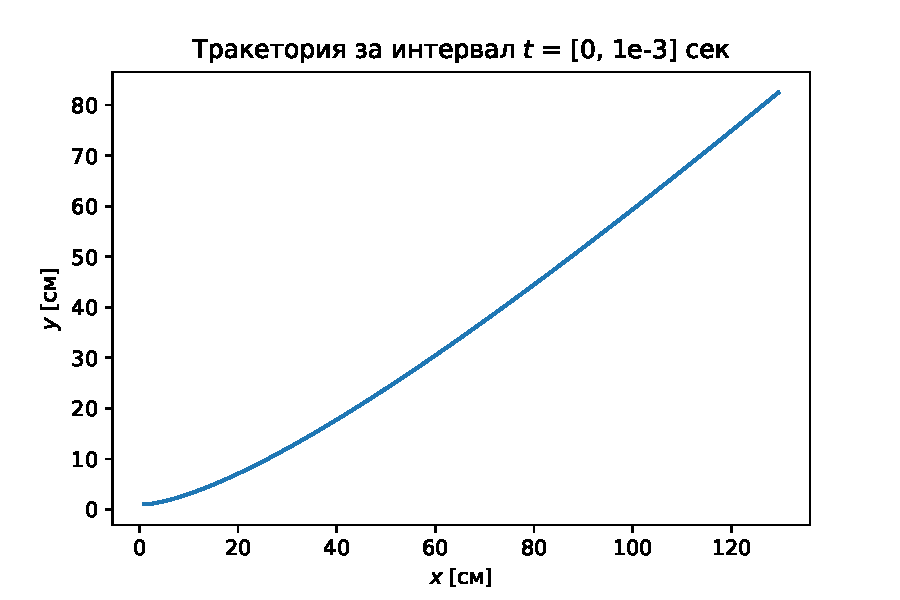
\includegraphics[width=\textwidth]{plotTrajectory.pdf}
	\caption{Электрон в электромагнитном поле. Геометрия задачи, начальные условия.}
	\label{graph_t}
\end{figure}

\begin{figure}

	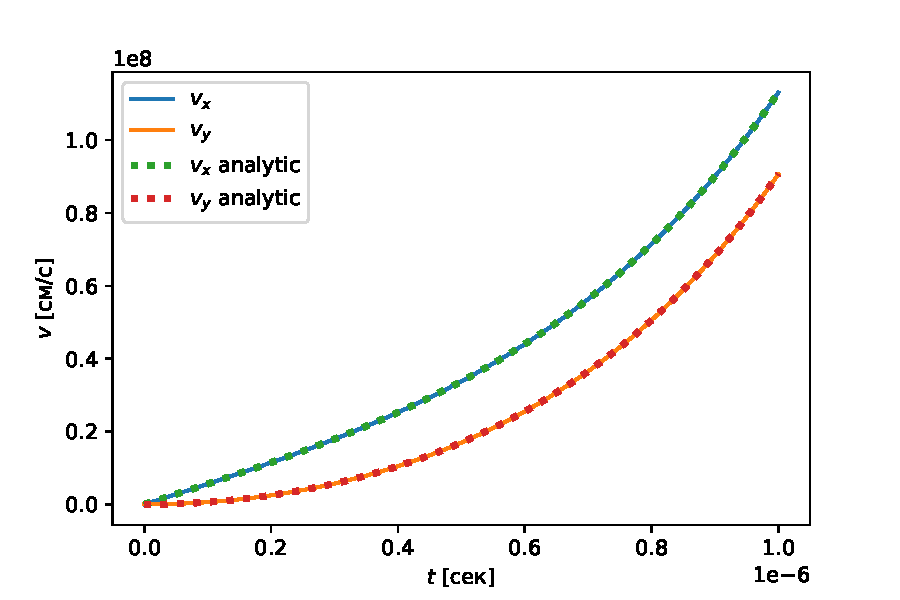
\includegraphics[width=\linewidth]{plotSpeed.pdf}
	\caption{Электрон в электромагнитном поле. Геометрия задачи, начальные условия.}
	\label{graph_s}
\end{figure}

\newpage
\section{Код программы}\label{code}
\lstinputlisting[language=Python, firstline=1, lastline=32]{lab5.py}













\end{document} % Конец текста.